\documentclass[12pt]{article} % Feel free to change this

\usepackage{graphicx}
\usepackage{mathptmx}
\usepackage[margin=1in]{geometry}

\begin{document}

\title{ECE 350: Digital Systems Final Project Report}
\author{Nathaniel Brooke, Matthew Barbano, Jesse Yue} % Change this to your name
\date{April 24, 2018} % Change this to the date you are submitting
\maketitle

\section*{Duke Community Standard}

By submitting this \LaTeX{} document, I affirm that
\begin{enumerate}
    \item I understand that each \texttt{git} commit I create in this repository is a submission.
    \item I affirm that each submission complies with the Duke Community Standard and the guidelines set forth for this assignment.
    \item I further acknowledge that any content not included in this commit under the version control system cannot be considered as a part of my submission.
    \item Finally, I understand that a submission is considered submitted when it has been received by the server.
\end{enumerate}

\section{Describe the overall project design and specifications}
This project was designed to be an implementation of Super Smash Bros. It is a two-player game in which two characters, Bowser and Kirby, fight each other to incur damage. Features include two GameCube-style 3D printed controllers, circuitry to convert this into DE2 board input, a physics engine, attacks/collision detection (based on button input combinations), knockback, hit boxes, damage control/lives, a splash screen, and VGA to display the game.\\

The general specification of this project was to implement a digital system with signficant input and output functionality. For our implementation of Super Smash Bros, these specifications involved integrating the 3D printed controllers and associated circuitry with the DE2 FPGA, and outputting the appropriate information onto the VGA.\\

\section{Describe input and output}
\subsection{Input}
The main inputs of this project were the two GameCube-style controllers. There were several components to each. First, the casing for each was 3D printed in three parts (front, back, and inside holder for circuitry), and all of the buttons were 3D printed (A, B, Jump, Reset, D-pad, Grab Trigger, and Shield Trigger) and attached along with the Parallax two-axis joystick. The buttons inside were then soldered to ~15-20 cables, which were attached to another group of circuitry. This mainly consisted of four ADCs, one for each axis of each joystick (each controlling a potentiometer), and a connector to the GPIO allowing the ~15-20 cables to interface with the DE2 board. The overflow 14-pin GPIO connector was also used for overflow. Since nearly all pins were used, only the top four digital outputs were used for each ADC to save space. Additionally, this circuitry does not require any external function generator or power source other than the DE2 board; all power and clocks were implemented via GPIO pins. Finally, this circuitry includes outputs for the LEDs and rumble motor in each controller, including an AND gate buffer used to restore a full signal reduced by the motors drawing current.\\

The software used to interface with this hardware directs all of the input signals to the appropriate locations to be used in the game to be used in functions such as physics calculations (joystick position), collision/attack detection and response (buttons), game flow (reset), and other functionality. The output signals (LEDs and rumble motors) respond to damage incurred by attacks.

\subsection{Output}
The primary output of the full project was the VGA monitor used to display gameplay. This displays the two players, Bowser and Kirby, the background/stage (which are integrated together and can interact when the characters collide with the stage), the player scores, the remaining lives for each players, and the splash screen upon termination of gameplay.\\

One particularly invovled VGA feature was animations, which included different Bowser/Kirby images for walking left/right, jumping, crouching, and every attack (not only each button, but also combinations of buttons, such as side B, up B, and down B, as in the real Super Smash Brothers game). Other VGA-based features include the seven-segment display style for damage, multiple strategies for reducing image (mif file) size due to the limit memory on the DE2 board, and implementing transparent backgrounds for images (that is, making the background show through the image bounding box). 

\section{Changes you had to make to your processor}
The major change made to the processor was to connect registers as inputs and outputs to and from other parts of the project. This included both severing the input wires to some registers in the regfile and replacing them with wires from outside the processor, and connecting an additional wire from the outputs of some registers to other locations outside the processor. Some examples include registers for LED/rumble motor output signals, damage, player width and height, and more. Additionally, to make the compile time of the project reasonable, the branch predictor and multiplier in the processor were removed.\\

\section{Challenges you faced and how you overcame them}
1. With respect to the physics-oriented calculations, velocity and acceleration were sometimes quite challenging to update correctly. For example, because the processor clock was so rapid, many velocities and accelerations caused the characters to disappear off screen. The solution was to create a timer which slowed down the main clock, allowing acceleration to be calculated properly.\\

2. Since Super Smash Brothers includes more images with much higher resolution than many other projects, it was challenging to fit all of the information into mif files without exceeding the memory capacity of the FPGA. There were several solutions to this problem, including reducing the number of colors in images to 64 and compressing images horizontally in mif files while re-stretching them out in the VGA code.\\

3. For the controllers, perfecting the 3D printing took several tries. Particularly, some sizes were off on the initial try (such as with the triggers fitting into the main body), with was solved with simple remeasuring and reprinting. However, some challenges were not as easy to resolve, such as fitting all of the wires into the controller. Solving this required shortening many of the wires connecting the buttons to power.\\

4. For the buttons on the controllers, occasionally small signals falsely triggered buttons (possibly due to a long power wire controlling all of the buttons, or another issue). The solution was to write code to make switches not respond to extremely quick triggers, as these are likely noise and not true button presses.\\

\section{Any circuit diagrams, how you constructed them, and the rationale behind them}
Below is a circuit diagram for the controller I/O. It can be divided into three sections:\\
1) Four ADCs - Each of these ADCs convert the signal from the axis potentiometer of a joystick to an 8-bit digital signal. The address 000 is used (pins 22, 23, and 24) are tied to ground, and only the top four output bits (pins 18-22) are used as GPIO input due to the limited number of GPIO pins. Note also that the clock pin is an output pin from the processor and is a slowed version of the processor clock created in software.\\

2) All Pushbuttons - This represents the input (typically attack) buttons from the controller. They use a pull down resistor to keep the pin grounded when the switch is open, and pull the pin up when the switch is closed.\\

3) LEDs/Rumble Motors - This AND gate acts as a buffer to restore the full voltage signal at the AND gate output. This is necessary because the motor draws a significant amount of current.\\

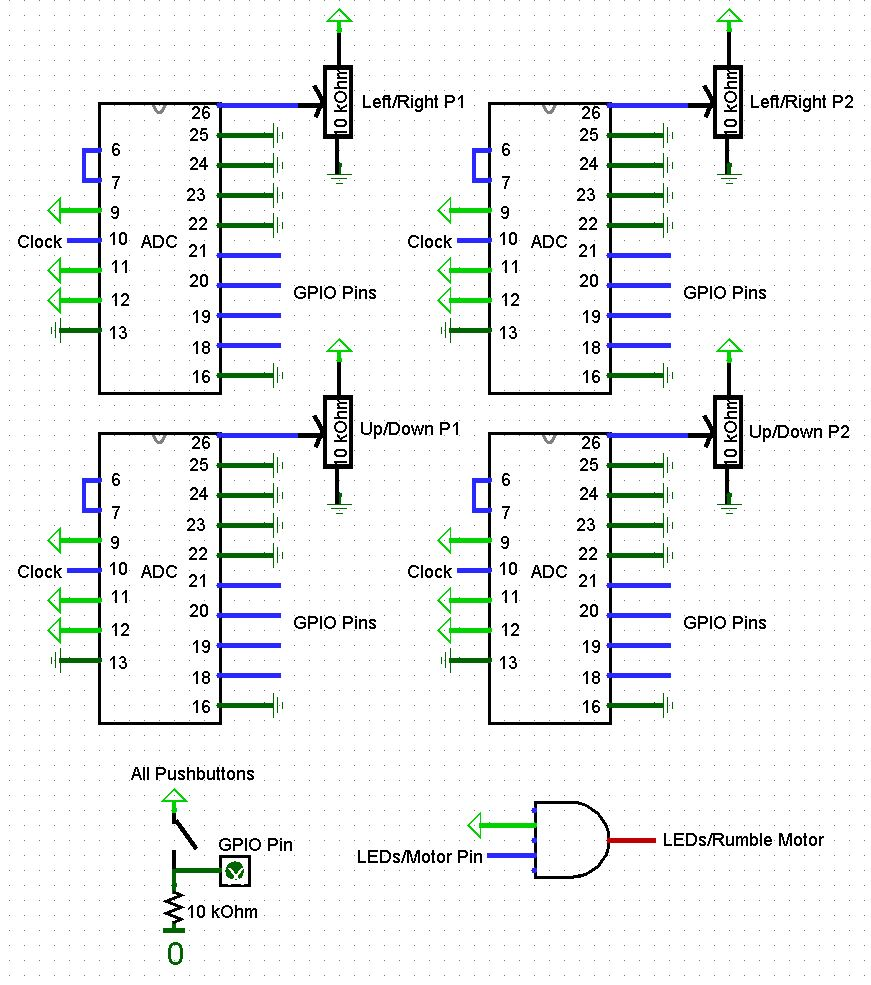
\includegraphics[scale=0.75]{circuit}\\


\section{Describe how you tested your project}
- Much of the debugging and testing occurred via visual observation of the VGA. Observing the location, velocity, and acceleration of characters allowed physics-based errors to be corrected, and observing which attack was executed when a given button combination was input allowed controller input and attacking to be debugged.\\

-  A particularly helpful testing method was to use the built-in LEDs on the VGA to display register or output values. One way this was used was to test the ADC inputs; a series of LEDs were wired to the digital input bits. They counted upwards when the control stick was moved from one extreme to the other. This approach was also used to test many other registers, storing values such as position, velocity, and attack combinations.\\

- To test the hardware, especially the four ADC circuits, a combination of strategies were employed. Multimeter testing and oscilloscope testing, including Digital Mode oscilloscope testing, were used to verify the correct operation of individual ADCs. To verify their correct wiring to the GPIO pins, the inputs were wired in Verilog to corresponding built-in LEDs on the DE2 board to test their correct operation without interference from game mechanics. Finally, game mechanics were integrated for a final check of the buttons.\\

- To test the assembly code, an isolated processor was often first used to debug via vector waveforms by wiring registers to the top level module and observing their values to see if they matched expected values.\\

\section{Describe your assembly programs or code}
Our assembly code performs several critical game functions. It performs calculations needed for the overall game flow, interacting both with modules geared more for input/output purposes and with clock-sensitive functionality. Some examples of assembly functionality include initializing constants used throughout the game, detecting attacks, responding to attacks (such as by blinking LEDs and signaling controller rumble motors), tracking player damage, decrementing player lives, and managing the splash screen.

\section{Flowchart of assembly code}
Below is a high-level flowchart of the assembly code.\\~\\
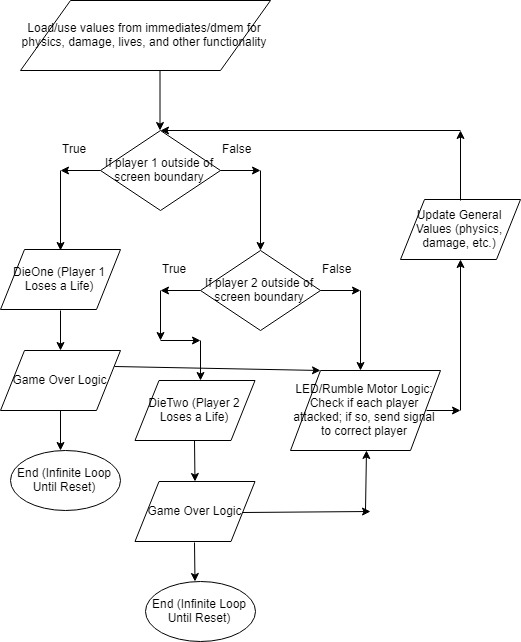
\includegraphics[scale=0.75]{flowchart}\\

\section{Pictures of your project}
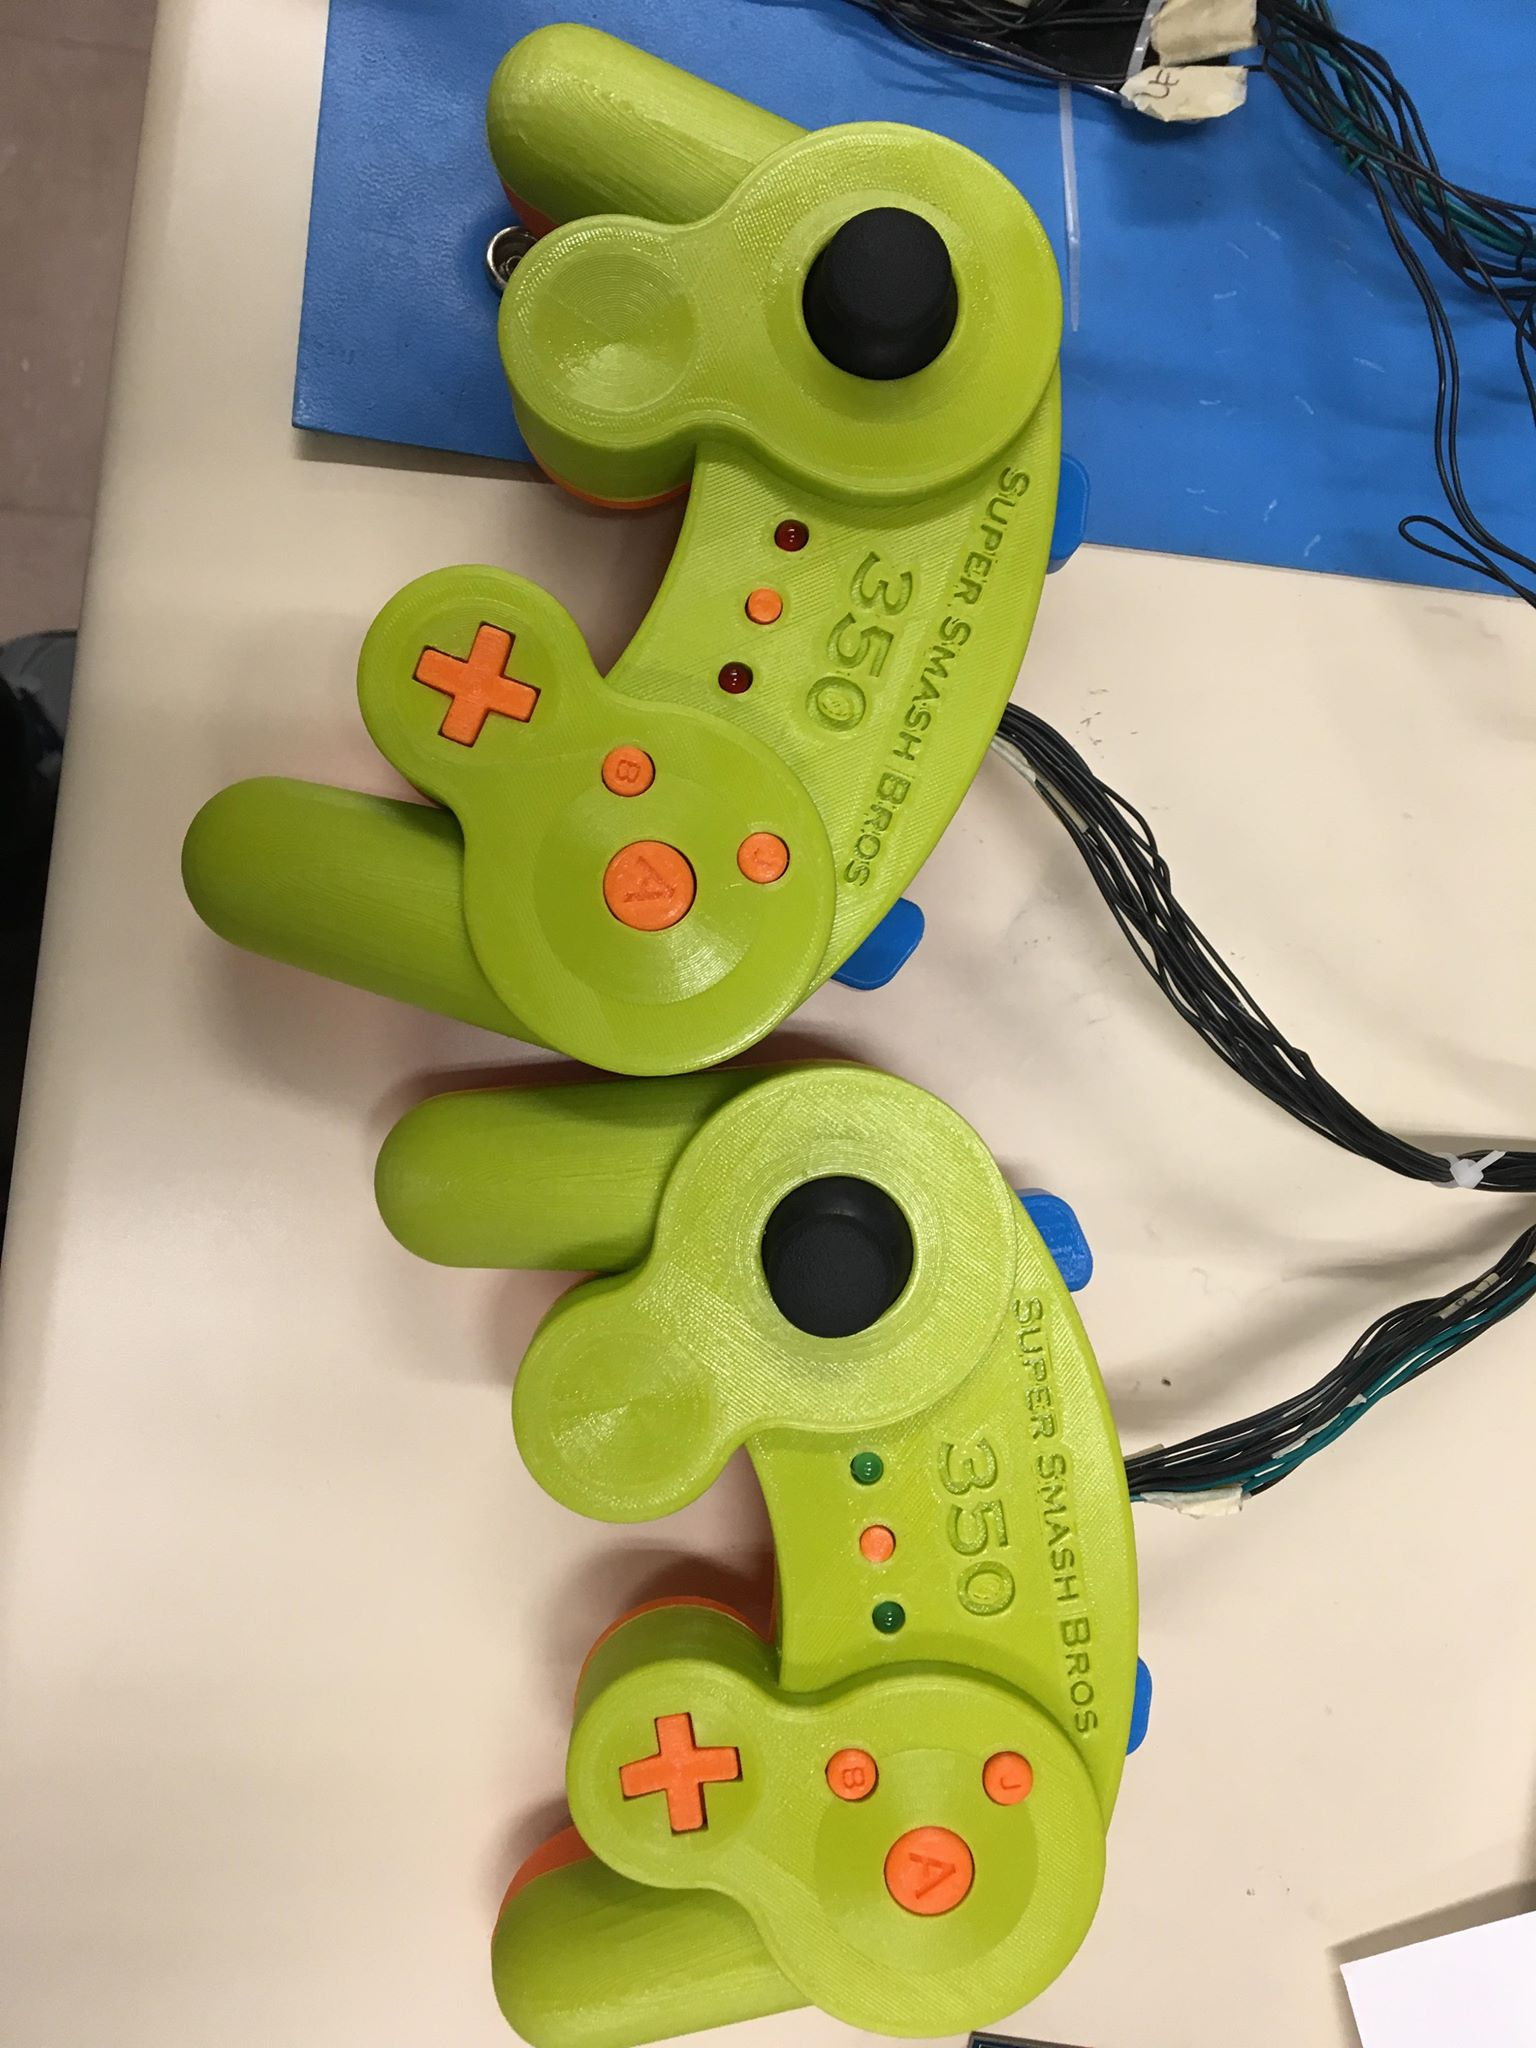
\includegraphics[scale=0.1]{pic1}\\
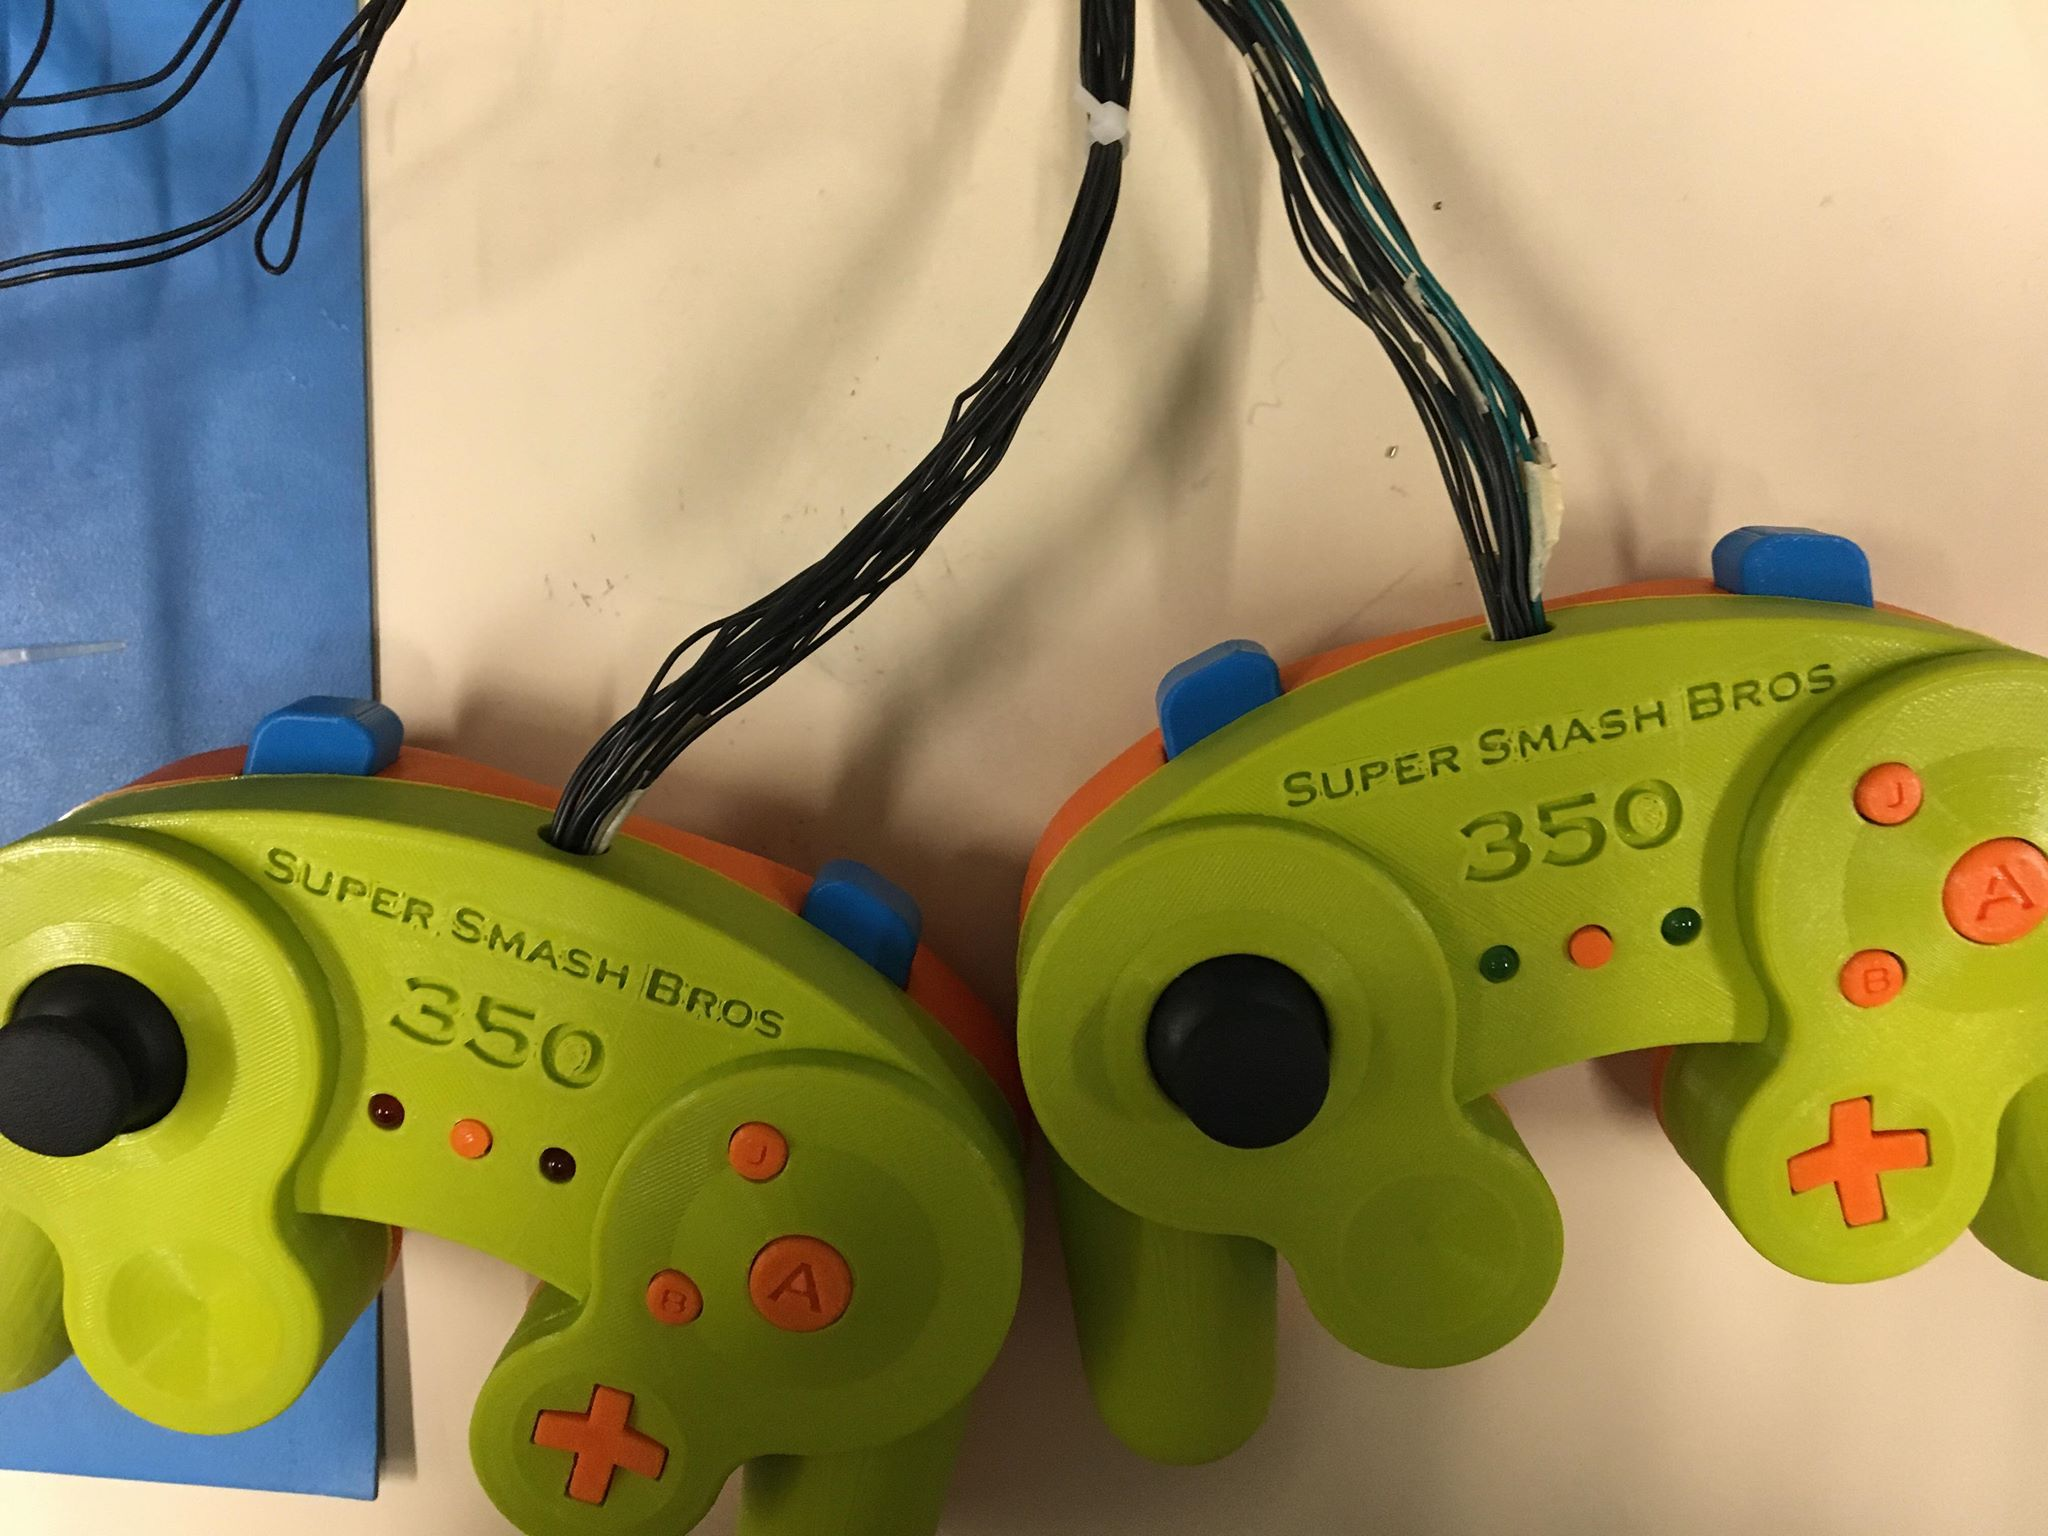
\includegraphics[scale=0.1]{pic2}\\
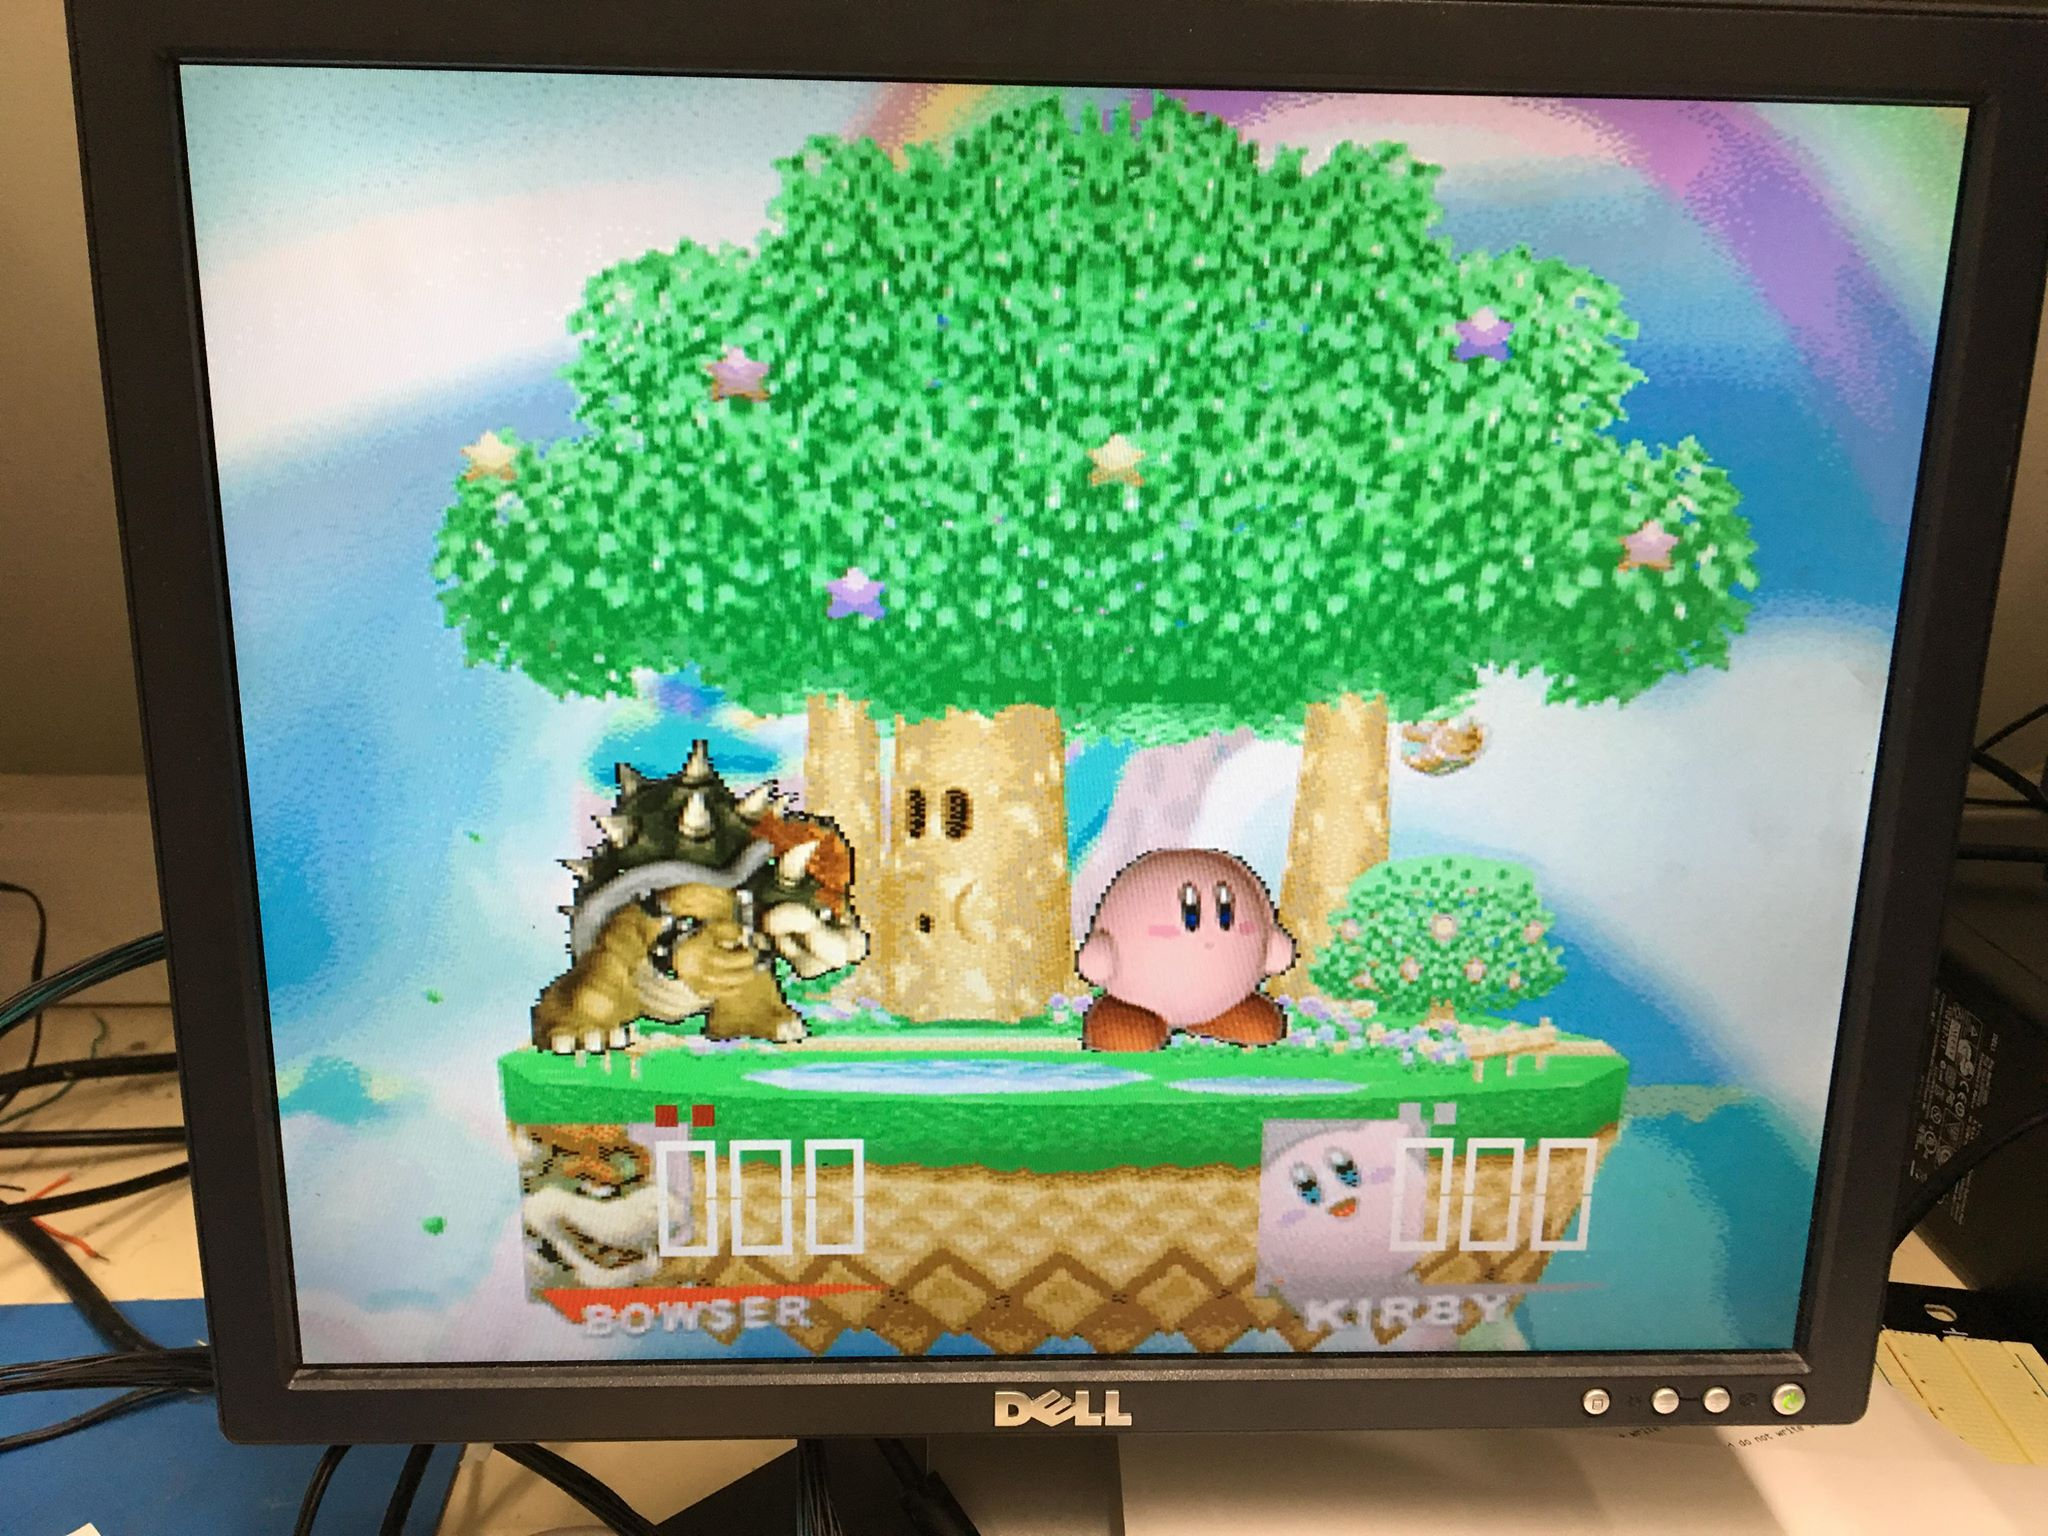
\includegraphics[scale=0.1]{pic3}\\
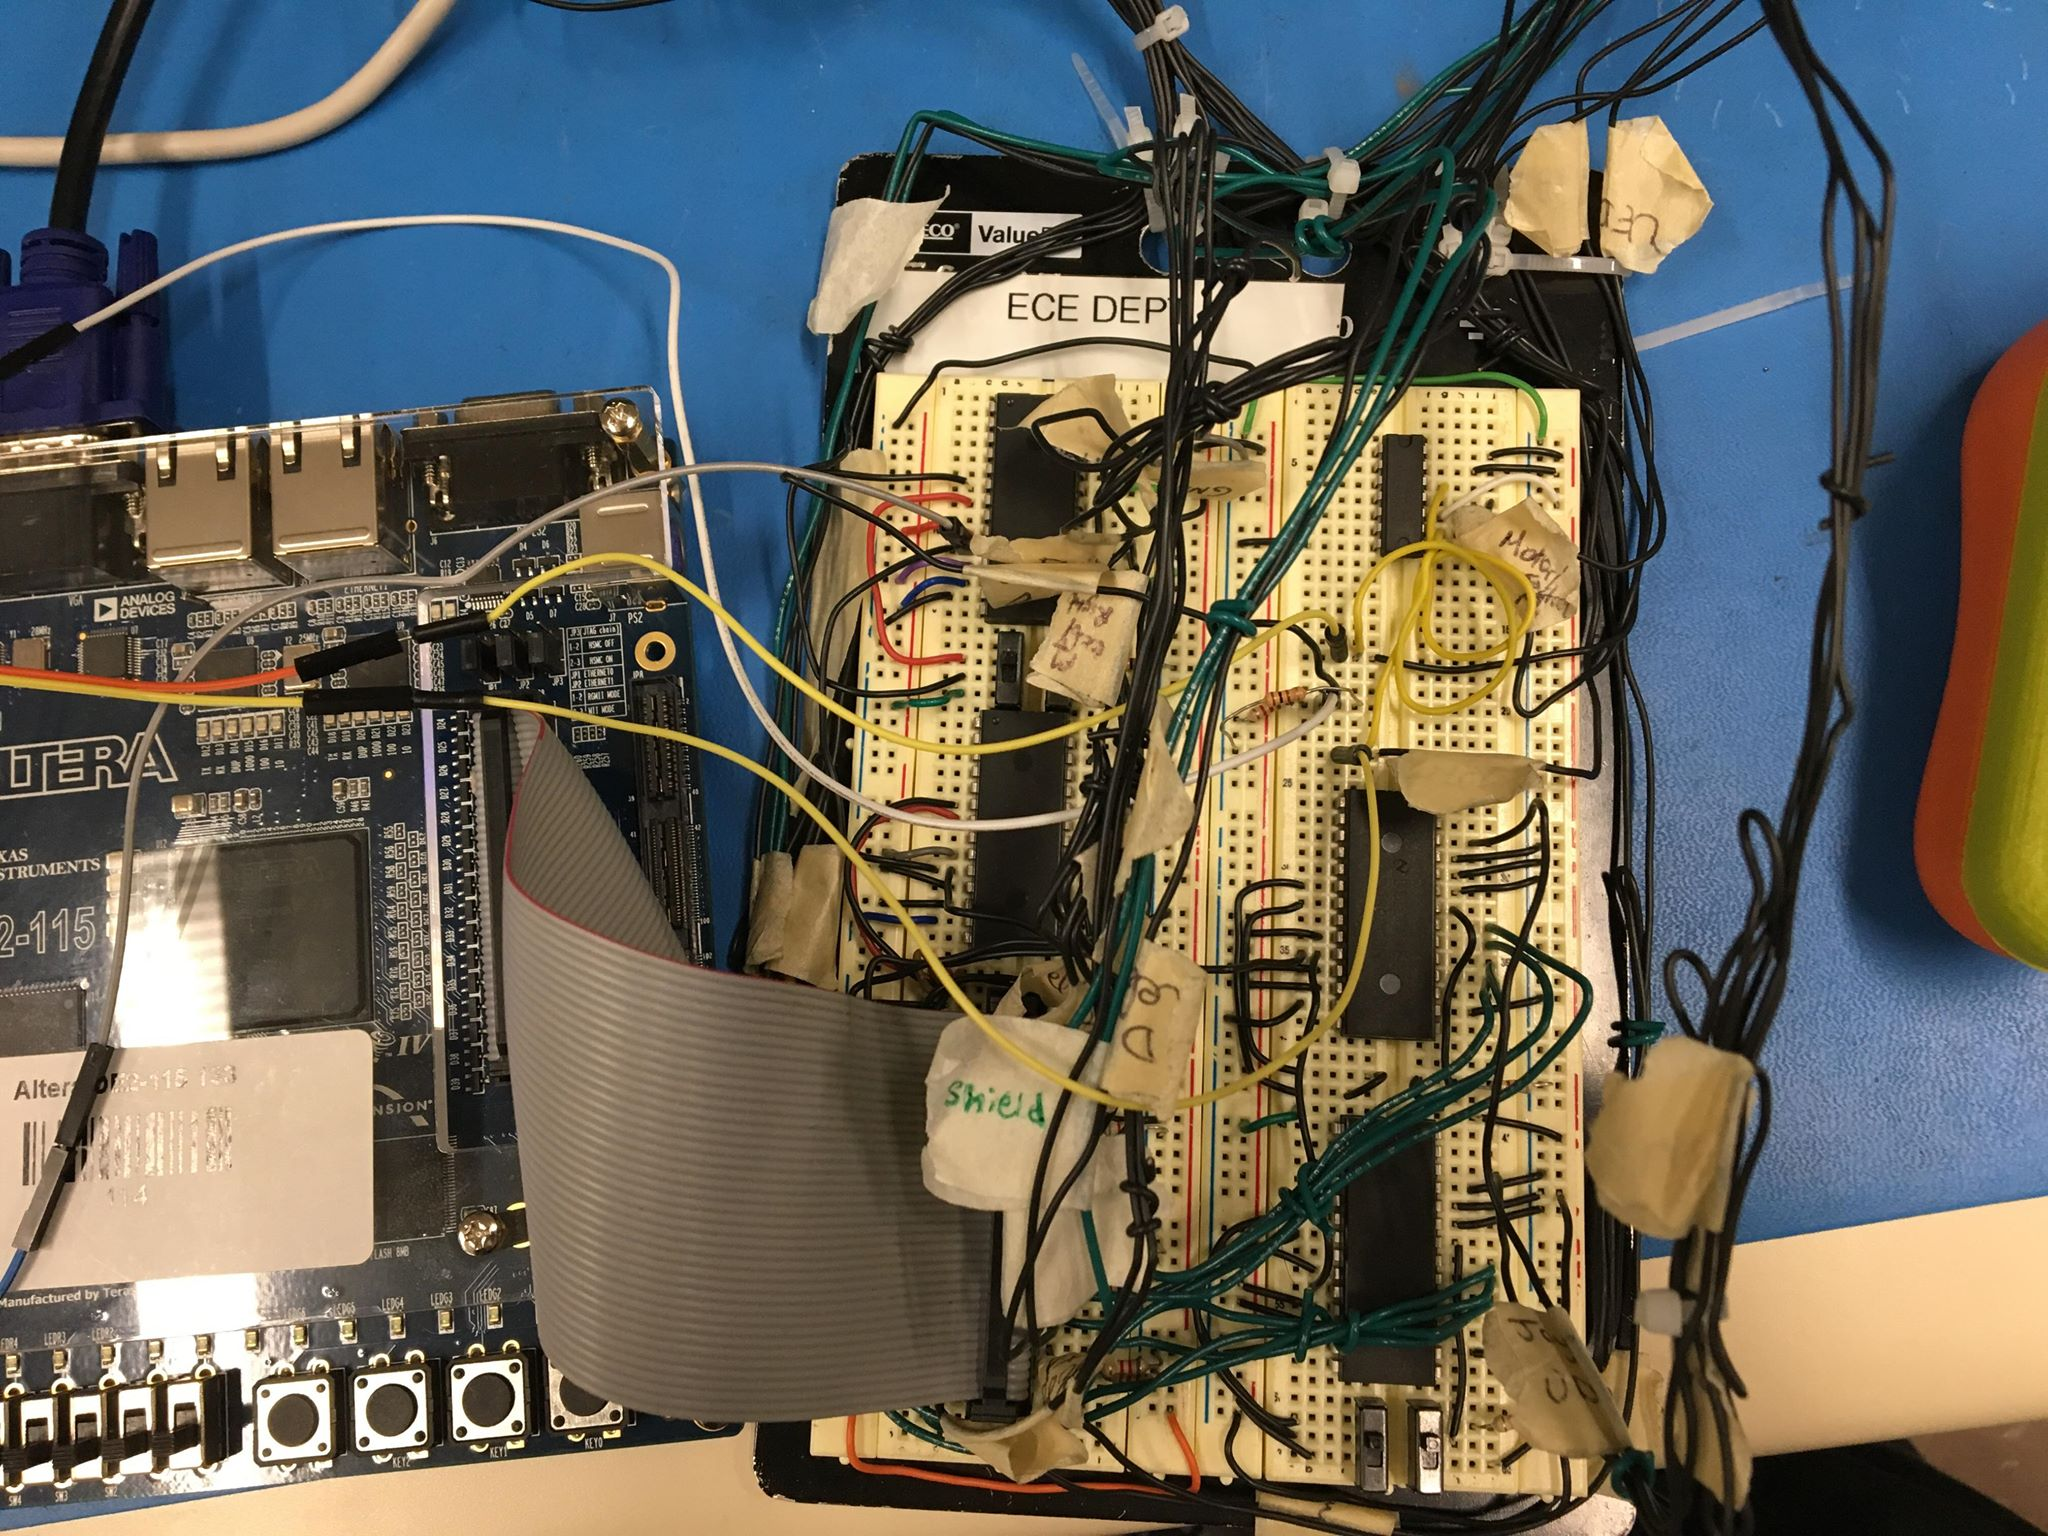
\includegraphics[scale=0.1]{pic4}\\
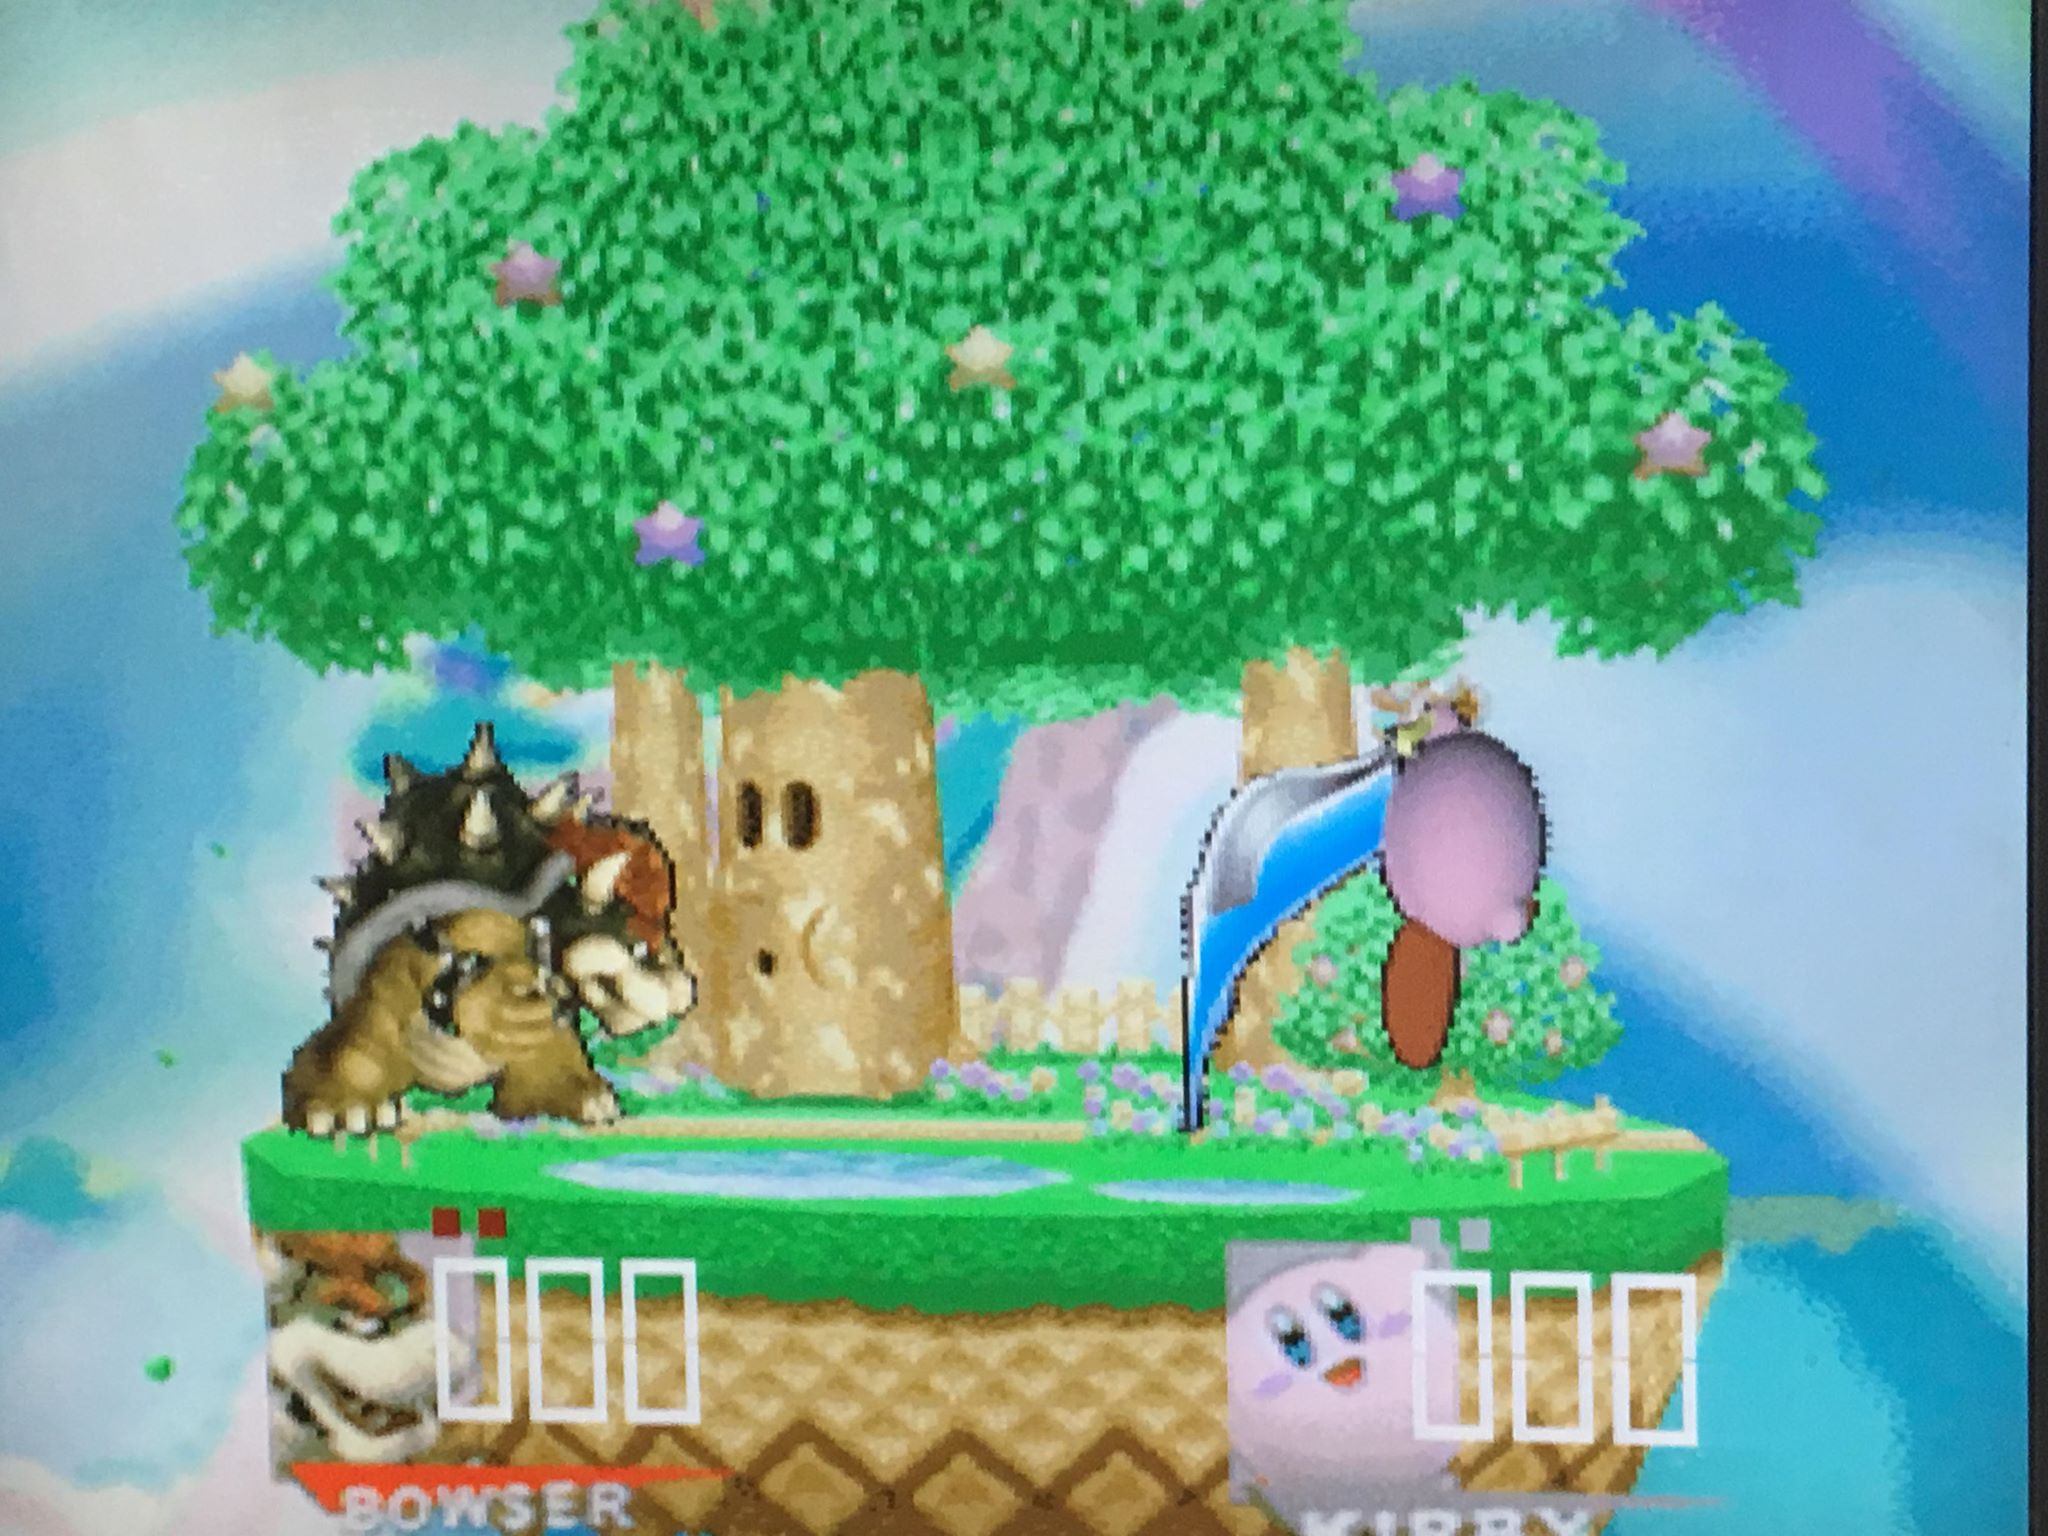
\includegraphics[scale=0.1]{pic5}\\
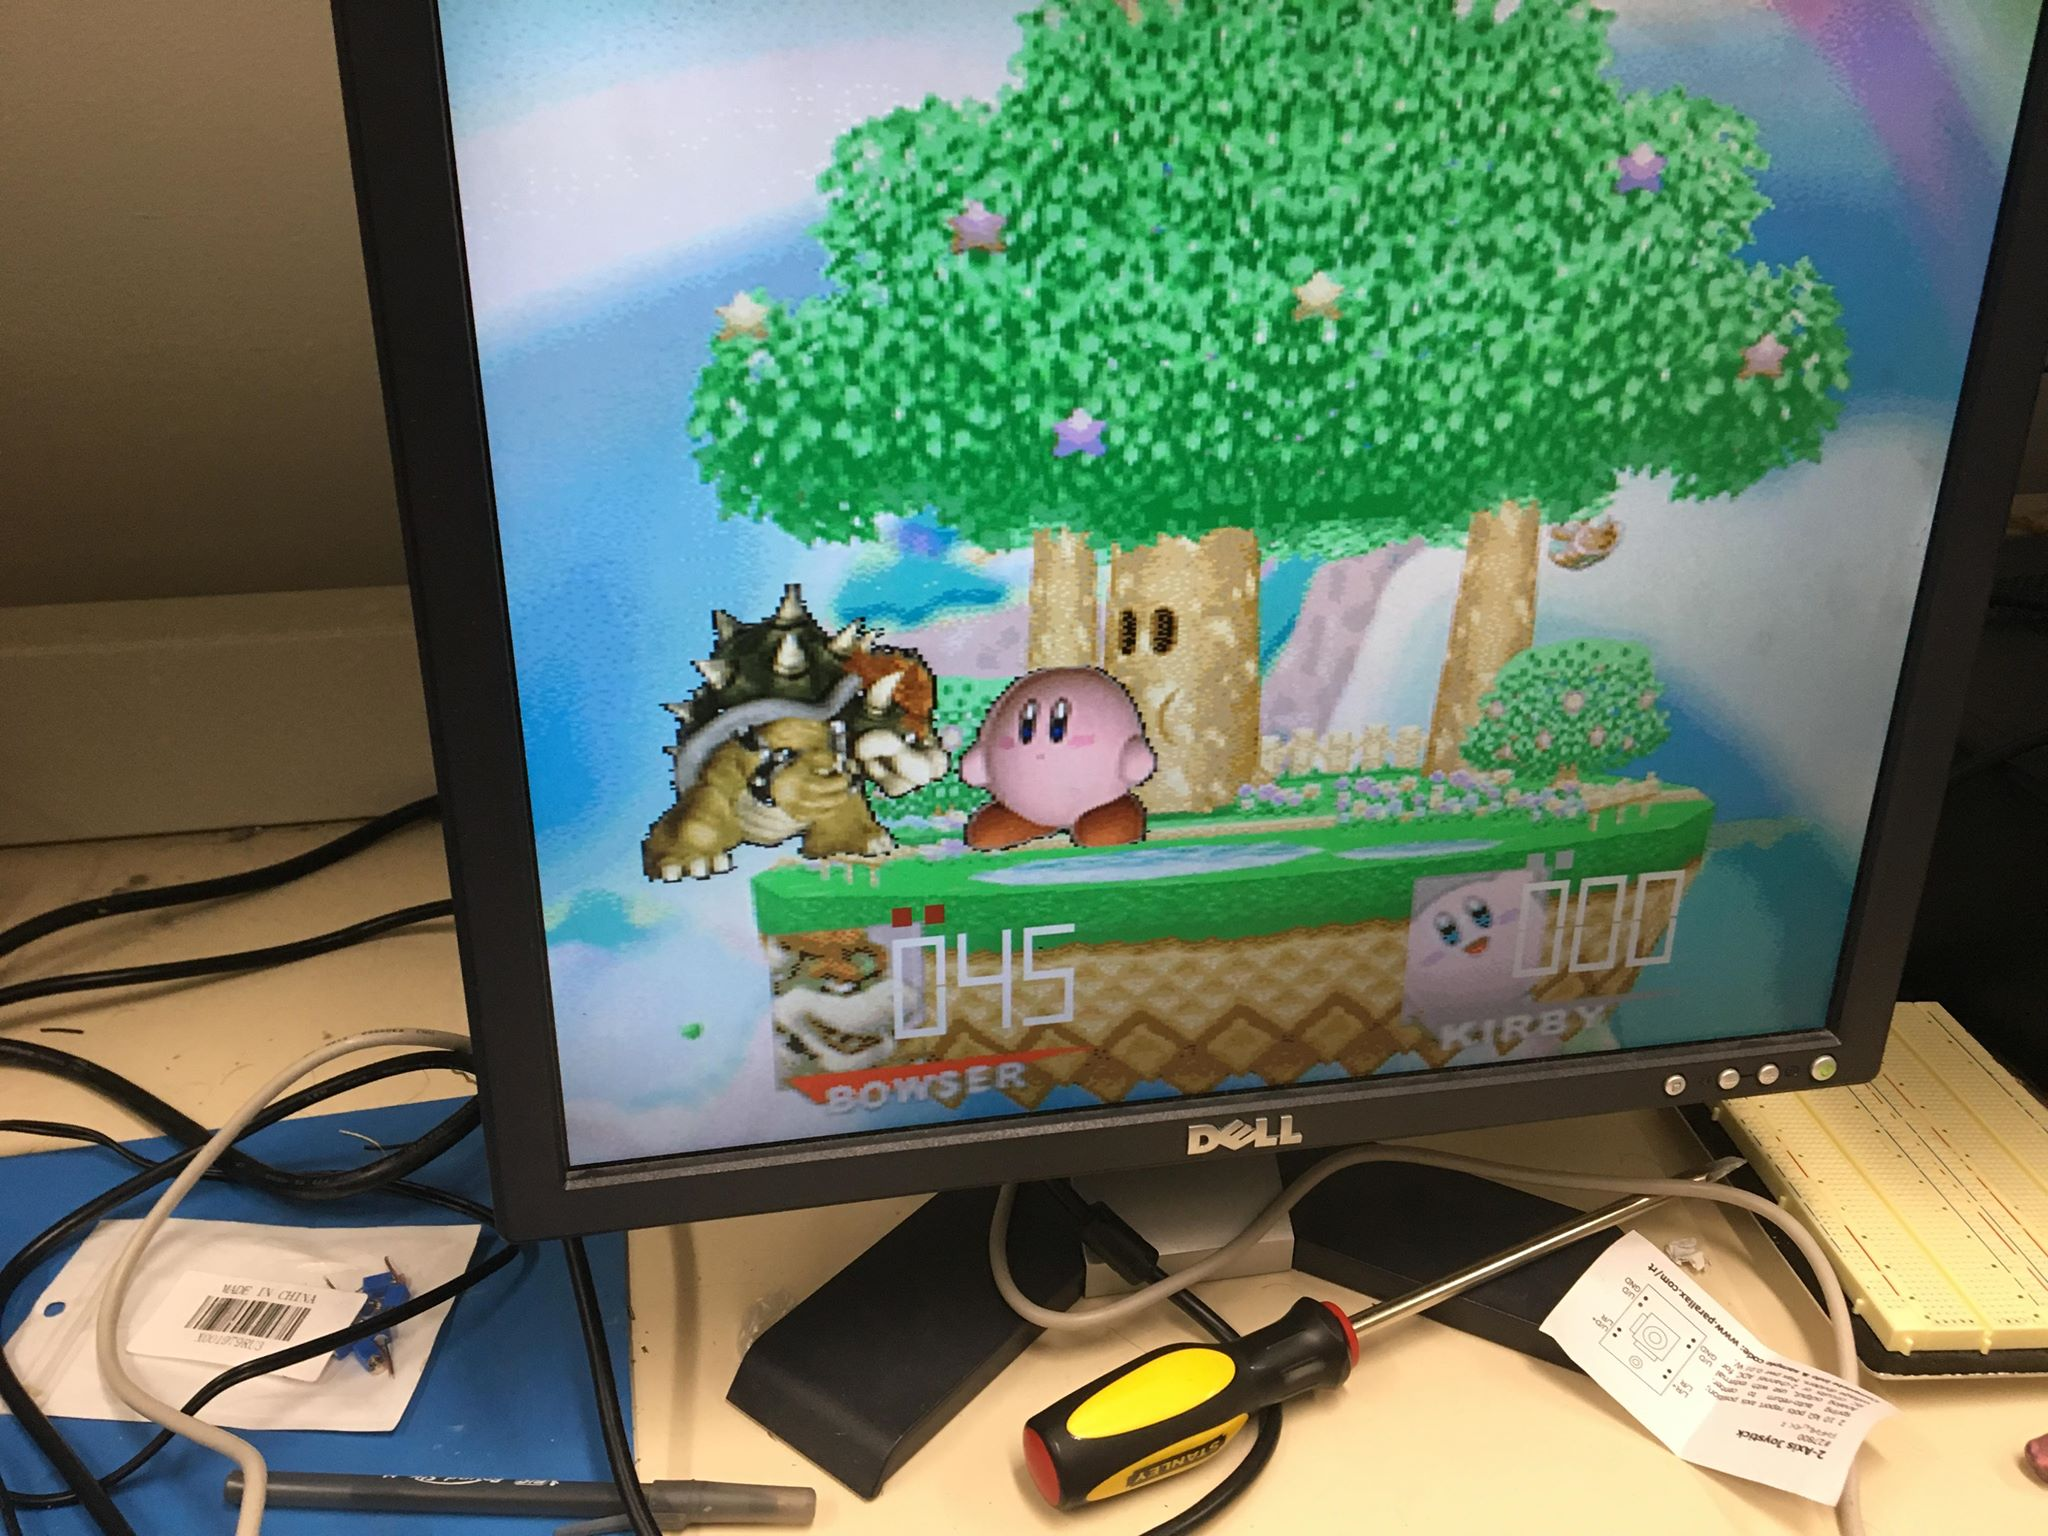
\includegraphics[scale=0.1]{pic6}\\

\end{document}